% artin2ord-c
% !TEX encoding = UTF-8 Unicode
% https://docs.google.com/document/d/1TzcpPwzt-dxjPA3za5ruDsuep48CUsZ3Cxy2xZBc3yE/edit?tab=t.0
% https://www.site24x7.com/tools/time-stamp-converter.html 1742999292
\documentclass[12pt,letterpaper]{article}
\usepackage{fancyhdr}
\fancyhf{}
\fancyfoot[R]{{\tiny artin2ord-b,\ \filemodprintdate{\jobname},\ \filemodprinttime{\jobname},\ 1742999292}} 
% https://latexonline.cc/ (doesn't work well; abandoned) - https://www.google.com/search?q=current+date+and+time
% (https://www.unixtimestamp.com/ bad) 
% LaTeX pense-bête https://docs.google.com/document/d/1kgwDp0rjOmd-9h5ryYvDeNTSUzUSdG13mo4ZNFToeYA/edit?tab=t.0
\renewcommand{\headrulewidth}{0pt}
\fancyfoot[C]{\thepage}
\usepackage[T1]{fontenc}
\usepackage[utf8]{inputenc}
\usepackage{amssymb,amsmath,amsthm} 
\usepackage[letterpaper,top=50pt,left=60pt,right=60pt,bottom=70pt]{geometry}
\usepackage{filemod}%https://stackoverflow.com/questions/2118972/latex-command-for-last-modified
\usepackage{microtype}
%\usepackage{comment}
\usepackage[pdfusetitle]{hyperref}%\texorpdfstring{$\boldsymbol{\tau_2}$}{tau2}
%\usepackage{marvosym}%\usepackage{showkeys}%\usepackage{showlabels}
%\usepackage[cal=boondoxo]{mathalfa}%https://tex.stackexchange.com/questions/479/lowercase-mathcal
%\usepackage[shortlabels]{enumitem}
\usepackage{tikz}
\pagestyle{fancy}
%\pagestyle{empty}
\setlength{\parskip}{5pt} % variable
%\renewcommand{\baselinestretch}{1.1} % variable
\newtheorem{thm}{Theorem}%[section]
%\newtheorem*{thm*}{Theorem}
%\newtheorem*{lem*}{Lemma}
\newtheorem{cor}[thm]{Corollary}
\newtheorem{lem}[thm]{Lemma}
\newtheorem{prop}[thm]{Proposition}
%\newtheorem*{prop*}{Proposition}
\newcommand{\aaa}{\mathcal a}\newcommand{\A}{\mathcal A}\newcommand{\B}{\mathcal B}\newcommand{\F}{\mathcal F}\newcommand{\SSS}{\mathcal S}\newcommand{\x}{\mathcal x}\newcommand{\y}{\mathcal y}
\newcommand{\ex}{\exists}\newcommand{\pt}{\forall}
\newcommand{\lra}{\leftrightarrow}\newcommand{\ra}{\rightarrow}
%\newcommand{\qa}{\bigtriangleup}\newcommand{\qb}{\bigtriangledown}
\newcommand{\noi}{\noindent}
\newcommand{\tf}{\therefore}
\newcommand{\g}{\gamma}
\newcommand{\mc}{\mathcal}
\newcommand{\R}{\mathbb R}

\begin{document}% \tiny \scriptsize \footnotesize \small \normalsize \large \Large \LARGE \huge \Huge 
%\begin{comment}
\begin{center}
{\Large Existence of a least increasing surjection from 

an artinian poset onto a set of ordinals\footnote{available at \url{https://github.com/Pierre-Yves-Gaillard/Artin-poset-to-ordinals}.}}\medskip 

{\small Pierre-Yves Gaillard}
\end{center}
%\end{comment}

\noi Let $X$ be a set. If $g:X\to S$ and $h:X\to T$ are surjections and $S$ and $T$ are sets of ordinals, say that $g\le h$ if $g(x)\le h(x)$ for all $x$. If $X$ is a poset, say that $g$ is \textbf{increasing} if $x<y$ implies $g(x)<g(y)$, and that it is \textbf{weakly increasing} if $x\le y$ implies $g(x)\le g(y)$. 

\begin{thm}\label{T1}
If $X$ is an artinian poset, then there is a least increasing surjection $f$ from $X$ onto a set of ordinals. 
\end{thm} 

The theorem will follow from Propositions \ref{P3} and \ref{P4} below. 

If $\beta$ is a ordinal, we write $[0,\beta)$ (resp. $[0,\beta]$) for the set of all ordinals $<\beta$ (resp. $\le\beta$). If $S$ is a set of ordinals, we denote by $\alpha(S)$ the least ordinal not in $S$, and by $\omega(S)$ the least ordinal larger than all the elements of $S$. We obviously have $\alpha(S)\le\omega(S)$. 

\begin{lem}\label{L2} 
The following conditions are equivalent: 

\noi\emph{(a)} $\alpha(S)=\omega(S)$, 

\noi\emph{(b)} $S=[0,\beta)$ for some ordinal $\beta$, 

\noi\emph{(c)} $S=[0,\alpha(S))$, 

\noi\emph{(d)} $S=[0,\omega(S))$, 

\noi\emph{(e)} no element of $S$ is larger than $\alpha(S)$. 
\end{lem}

The proof is left to the reader. 

Recall that $X$ is an artinian poset. For $x$ in $X$, set $X_x:=\{y\in X\ |\ y<x\}$. Let $\kappa$ be a cardinal larger that the cardinality of $X$, and set $A:=[0,\kappa]$. For $x$ in $X$ let $A^{X_x}$ be the set of all maps from $X_x$ to $A$. Define $r_x:A^{X_x}\to A$ by letting $r_x(h)$ be the minimum of $\kappa$ and $\alpha(h(X_x))$, and $s_x:A^{X_x}\to A$ by letting $s_x(h)$ be the minimum of $\kappa$ and $\omega(h(X_x))$. If $h:X\to A$ is a map, we denote by $h|X_x$ the restriction of $h$ to $X_x$. By the last statement in 

\url{https://github.com/Pierre-Yves-Gaillard/The-Transfinite-Recursion-Theorem}

\noi there is a unique map $f:X\to A$ such that $f(x)=r_x(f|X_x)$ for all $x$ in $X$, and a unique map $g:X\to A$ such that $g(x)=s_x(g|X_x)$ for all $x$ in $X$. For all $x$ in $X$ set $\alpha_x:=\alpha(f(X_x))$ and $\omega_x:=\omega(g(X_x))$.

\begin{prop}\label{P3} 
We have: 

\noi\emph{(f)} $f=g$, 

\noi\emph{(g)} $f(X_x)=[0,\alpha_x)=[0,\omega_x)$ for all $x$. 

\noi\emph{(h)} $f(x)=\alpha_x=\omega_x$ for all $x$. 
\end{prop} 

\begin{proof} 
Note that $f$ and $g$ are weakly increasing. Let (f') be the condition (obviously equivalent to (f)) that $f(x)=g(x)$ for all $x$. Assume by contradiction that at least one of the three conditions (f'), (g), (h) is false. Let $x$ be minimal among the elements for which (f'), (g) or (h) fails. Note that $f(X_y)=g(X_y)$ for $y\le x$. %, and set $\alpha_y:=\alpha(f(X_y))$ and $\omega_y:=\omega(f(X_y))$. 

% previous versions https://docs.google.com/document/d/1NIxqDHrGcBNod-Qx1hGy-WhRdYl3dwIO36OppiXpS-Y/edit?tab=t.0
We have $\alpha_x\le\omega_x$. If $\alpha_x=\omega_x$, then the lemma implies $f(X_x)=[0,\alpha_x)$, and (f'), (g) and (h) hold for $x$, contradiction. We conclude that $\alpha_x<\omega_x$. By (e) there is a $y$ less than $x$ such that $f(y)>\alpha_x\notin f(X_x)$. %Let $z$ be less than $y$. 

\noi Claim: We have $f(z)<\alpha_x$ for $z<y$. 

\noi Proof: Otherwise we would have $\alpha_x<f(z)$, and thus  
$$
\alpha_x\in[0,f(z))=[0,\alpha_z)=[0,\omega_z)=f(X_z)\subset f(X_x),
$$ 
contradiction. This proves the claim. 

By the claim $\alpha_x$ is larger than each element of $f(X_y)$, hence $\alpha_x\ge\omega_y$, hence $f(y)=\omega_y\le\alpha_x<f(y)$, contradiction. 
\end{proof} 

\begin{prop}\label{P4} 
We have: 

\noi\emph{(i)} $f(X)=[0,\alpha(f(X)))=[0,\omega(f(X)))$, 

\noi\emph{(j)} $f:X\to[0,\alpha(f(X)))$ is the least increasing surjection from $X$ onto a set of ordinals. 
\end{prop} 

\begin{proof}
Define the poset $Y$ be the following conditions: $Y=X\cup\{\infty\},\infty\notin X,X$ is a sub-poset of $Y$. Then $Y$ is artinian and satisfies $Y_\infty=X$, and we can prove (i) by applying Proposition~\ref{P3} to $Y$ (instead of $X$). More precisely, let $f:X\to S$ (resp. $g:X\to S$) be the least increasing surjection from $X$ (resp. $Y$) onto a set of ordinals. We have $f(X)=g(X)=[0,\alpha(f(X)))=[0,\omega(f(X)))$, the first equality following from the fact that $Y_\infty=X$, the second and third equalities following from (g) above. %Recalling that $Y_\infty=X$, we see that $f$ and $g$ coincide on $X$, and we get $f(X)=g(X)=[0,\alpha(f(X)))=[0,\omega(f(X)))$. 
Then (j) is a consequence of (i) and Proposition~\ref{P3}. 
\end{proof} 

The following corollary to Propositions \ref{P3} and \ref{P4} is well known. 

\begin{cor}
Let $\beta$ be an ordinal, $X$ a subset of $[0,\beta)$ and $f:X\to[0,\gamma)$ the least increasing surjection of $X$ onto a set of ordinals. Then we have $f(x)\le x$ for all $x$, and $\gamma\le\beta$. 
\end{cor} 

\begin{proof}
It suffices to show $f(x)\le x$ for all $x$. Suppose not, and let $x$ be the least element of $X$ satisfying $f(x)>x$. We get $x<f(x)=\alpha(f(X_x))=\omega(f(X_x))$ and $f(X_x)=[0,f(x))\ni x$, hence $x=f(y)$ for some $y$ less than $x$, hence $f(y)\le y<x=f(y)$, contradiction. 
\end{proof} 

%\newpage

We end with a loosely related question. If $X$ and $Y$ are posets and $f:X\to Y$ and $g:Y\to X$ are increasing surjections, are $X$ and $Y$ necessarily isomorphic? The following example shows that the answer is no. Let $X$ and $Y$ be the posets respectively given by the Hasse diagrams 
$$
\begin{tikzpicture}[scale=.5]
  \node (b1) at (-3,0) {$b_1$};
  \node (b2) at (-1,0) {$b_2$};
  \node (b3) at (1,0) {$b_3$};
  \node (a1) at (-3,-2) {$a_1$};
  \node (a2) at (-1,-2) {$a_2$};
  \node (a3) at (1,-2) {$a_3$};
  \node (e) at (3,-1) {$\cdots$};
  \draw (b1) -- (a1) (b2) -- (a2) (b3) -- (a3);
\end{tikzpicture}
$$ 
and
$$
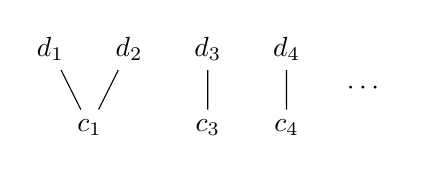
\begin{tikzpicture}[scale=.5]
  \node (d1) at (-3,0) {$d_1$};
  \node (d2) at (-1,0) {$d_2$};
  \node (d3) at (1,0) {$d_3$};
  \node (d4) at (3,0) {$d_4$};
  \node (c1) at (-2,-2) {$c_1$};
  \node (c3) at (1,-2) {$c_3$};
  \node (c4) at (3,-2) {$c_4$};
  \node (e) at (5,-1) {$\cdots$};
  \draw (d1) -- (c1) -- (d2) (d3) -- (c3) (d4) -- (c4);
\end{tikzpicture}
$$ % previous version https://docs.google.com/document/d/1ez4akBT2g96p8B-LpPlzpSYqdCD_D-gWmsRy9ZpUxfw/edit?tab=t.0
We see that if we identify $a_1$ and $a_2$ in $X$ we get a poset isomorphic to $Y$, and if we identify $d_1$ and $d_2$ in $Y$ we get a poset isomorphic to $X$. 

\end{document}
